\chapter{Informatik -- Worum geht's?}
\renewcommand{\chaptertitle}{Informatik -- Worum geht's}

\lehead[]{\sf\hspace*{-2.00cm}\textcolor{white}{\colorbox{lightblue}{\makebox[1.60cm][r]{\thechapter}}}\hspace{0.17cm}\textcolor{lightblue}{\chaptertitle}}
\rohead[]{\textcolor{lightblue}{\chaptertitle}\sf\hspace*{0.17cm}\textcolor{white}{\colorbox{lightblue}{\makebox[1.60cm][l]{\thechapter}}}\hspace{-2.00cm}}
%\chead[]{}
\rehead[]{\textcolor{lightblue}{AvHG, Inf, My}}
\lohead[]{\textcolor{lightblue}{AvHG, Inf, My}}


\section{Informatik}

\subsection{Gegenstand der Informatik}

Die meisten Menschen denken bei Informatik sofort an Computer. Nicht ganz zu
Unrecht, denn Computer sind als Werkzeug für die Informatik von zentraler Bedeutung.

Dem gegenüber steht ein bekanntes Zitat des niederländischen Informatikers
Edsger Wybe Dijkstra:

\begin{quotation}
\noindent In der Informatik geht es genauso wenig um Computer wie in der
Astronomie um Teleskope.
\end{quotation}

Auch hier wird auf den Werkzeugcharakter des Computers hingewiesen.

Die Informatik beschäftigt sich als Wissenschaft mit der automatisierten
Informationsverarbeitung. Um Informationen automatisiert verarbeiten zu können
braucht es zum einen entsprechende Maschinen (Computer) und zum anderen genaue
und eindeutige Handlungsanweisungen, mit deren Hilfe die Daten der jeweiligen
Aufgabenstellung entsprechend verarbeitet werden können.

Eine solche eindeutige Handlungsanweisung zur Lösung eines Problems wird
\emph{Algorithmus} genannt. Dies ist ein zentraler Begriff in der Informatik.


\subsection{Teilgebiete der Informatik}

\begin{figure}[h]
  \centering
   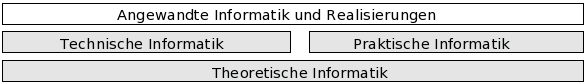
\includegraphics[width=1.0\textwidth]{./inf/SEKII/03_Informatik/Architektur-der-Informatik.png}
   \caption{Teilgebiete der Informatik}
   %
   % http://de.wikipedia.org/wiki/Informatik#mediaviewer/Datei:Architektur-der-informatik.png, Erstellt von Matthias Kleine. Lizenziert unter Creative Commons Attribution-Share Alike 3.0
\end{figure}
% http://de.wikipedia.org/wiki/Informatik#mediaviewer/Datei:Architektur-der-informatik.png

Im Informatikunterricht werden wir uns schwerpunktmäßig mit Themen der
\emph{Praktischen Informatik} beschäftigen (mit anderen Worten: Ihr werdet
lernen passende Algorithmen für gegebene Probleme zu finden und diese zu
implementieren/programmieren).

Aber auch Themen aus den anderen Teilgebieten der Informatik werden wir
behandeln:

\begin{compactitem}
\item[\emph{Theoretische Informatik}:]\hspace{1cm}
  \begin{compactitem}
  \item Aussagenlogik
  \item Kryptologie
  \end{compactitem}
\item[\emph{Technische Informatik}:]\hspace{1cm}
  \begin{compactitem}
  \item Rechnerarchitektur
  \item Aufgaben und Funktionsweise von Betriebssystemen
  \item Netzwerkprotokolle
  \end{compactitem}
\item[\emph{Angewandte Informatik}:]\hspace{1cm}
  \begin{compactitem}
  \item Datenschutz und Urheberrecht
  \item Informatik und Gesellschaft
  \item Anwendungsgebiete in Wirtschaft und Wissenschaft
  \end{compactitem}
\end{compactitem}


\section{Was Computer können}

Computer können nur zwei Dinge tun:

\begin{compactenum}[1.]
\item Berechnungen ausführen.
\item Sich die Ergebnisse solcher Berechnungen merken. 
\end{compactenum}

Das ist tatsächlich nicht viel. Diese zwei Dinge können Computer allerdings
\emph{sehr} gut! Ein typischer PC führt pro Sekunde eine Milliarde
Rechenoperationen aus. Selbst in der unvorstellbar kurzen Zeit, die Licht
braucht um von der Schreibtischlampe auf eine nur 60 Zentimeter entfernte
Schreibtischoberfläche zu gelangen, hat der PC bereits zwei Berechnungen
durchgeführt. Und dabei ist Licht wirklich verdammt schnell: Pro Sekunde legt
Licht eine Entfernung von dreihunderttausend Kilometern zurück. Mit dieser
Geschwindigkeit kann man die Erde in einer Sekunde acht Mal umkreisen!

Während des überwiegenden Teils der Menschheitsgeschichte waren die
Möglichkeiten, Berechnungen anzustellen und deren Ergebnisse festzuhalten,
durch die Leistungsfähigkeit des menschlichen Gehirns beschränkt. Das bedeutete,
dass nur die kleinsten und einfachsten durch Berechnung zu lösenden Probleme
angegangen werden konnten. Selbst mit der Geschwindigkeit moderner Computer
bleiben noch unlösbare Probleme. Zum Beispiel die langfristigen Wetter- und
Klimavorhersagen. Aber mit der der zunehmenden Leistungsfähigkeit der Computer
werden mehr und mehr Problemstellungen einer Lösung mit Hilfe von Computern
zugänglich.

Zwar kann der Computer nur mit Zahlen rechnen (genau genommen nur mit Null und
Eins), aber auch Buchstaben, Ton, Bild, Wetterdaten -- ganz Allgemein:
\emph{Informationen} -- lassen sich als Zahlen darstellen. Und somit auch
berechnen.


\section{Computational Thinking}

\emph{Computational Thinking} ist ein relativ neuer Begriff in der Informatik.
Beschrieben wird damit die Fähigkeit, auch alltägliche Problemstellungen
daraufhin zu untersuchen, ob und wie man sie mit Hilfe von Computern lösen
könnte.

Populär wurde der Begriff durch Jeannette Wing, Leiterin des Computer Science
Departments an der Carnegie Mellon University in Pittsburgh (USA).

Zitat aus einem Artikel in der österreichischen Tageszeitung \emph{Der Standard}
vom 28.\ September 2010:

\begin{quotation}
\noindent Wer analytisch und präzise wie ein Computerwissenschafter denken
lernt, kann komplexe Probleme effizienter lösen.

\noindent Mit dem Denkmodell könnten selbst alltägliche Aufgaben wie das
Kaffeeholen in der Cafeteria effizienter gestaltet werden. Den Unterschied zu
gewissermaßen \glqq herkömmlichem\grqq\ logischem Denken erklärt Wing mit dem
herausragenden Stellenwert von Effizienz in der Computerwissenschaft:
\glqq Computational Thinking befähigt dazu, Strukturen und Muster zu erkennen,
wo man vorher keine gesehen hat, oder effizienter in der täglichen Routine zu
sein.\grqq

\noindent Besonderes Augenmerk legt die Wissenschaftlerin auf die
Implementierung ihres Konzeptes in das Bildungswesen. \glqq Zusätzlich zu den
Fertigkeiten wie Schreiben, Rechnen und Lesen sollte in Zukunft jedes Kind als
weitere analytische Fähigkeit die grundlegenden Konzepte der
Computerwissenschaften verinnerlichen\grqq .

\noindent \glqq Wenn wir lernen, schriftlich zu dividieren oder zwei große
Zahlen zu multiplizieren, lernen wir eigentlich einen Algorithmus. Nur sagt uns
das niemand\grqq , so Wing.
\end{quotation}

Quelle: \url{http://derstandard.at/1285199497847/}




